\documentclass[11pt]{article}
\usepackage[margin=1in]{geometry}
\usepackage{amsmath,amssymb,amsfonts,bm,mathtools}
\usepackage{tikz}
\usetikzlibrary{arrows.meta,positioning,shapes.geometric}
\usepackage{hyperref}

\title{Hyperbolic VAE: Rigorous Mathematical Formulation}
\date{}

\begin{document}
\maketitle

\section{Latent manifold}
For curvature magnitude $c>0$, the latent space is the Poincar\'e ball
\begin{equation}
\mathbb B_c^d=\{u\in\mathbb R^d:\,c\|u\|_2^2<1\},
\end{equation}
with constant curvature $-c$. The metric is
\begin{equation}
g_u=\lambda_u^2 I_d,
\qquad
\lambda_u=\frac{2}{1-c\|u\|_2^2}.
\end{equation}
At the origin, $T_0\mathbb B_c^d\cong\mathbb R^d$.

\section{Variational posterior in tangent space}
Given input $x\in\mathbb R^p$, the encoder outputs $(\mu_\phi(x),\log\sigma_\phi^2(x))$ and defines
\begin{equation}
q_\phi(v\mid x)=\mathcal N\big(\mu_\phi(x),\operatorname{diag}(\sigma_\phi^2(x))\big),
\qquad v\in T_0\mathbb B_c^d.
\end{equation}
Sampling uses reparameterization:
\begin{equation}
v=\mu_\phi(x)+\sigma_\phi(x)\odot\varepsilon,
\qquad \varepsilon\sim\mathcal N(0,I_d).
\end{equation}
Map to manifold:
\begin{equation}
z=\exp_0^{\mathbb B_c}(v),
\end{equation}
followed by projection for numerical stability.

\section{Origin maps}
With $r=\|v\|_2$, the origin exponential map is
\begin{equation}
\exp_0^{\mathbb B_c}(v)=\tanh(\sqrt c\,r)\frac{v}{\sqrt c\,r},
\end{equation}
with continuous extension at $v=0$. For $z\in\mathbb B_c^d$, the origin logarithm map is
\begin{equation}
\log_0^{\mathbb B_c}(z)
=\frac{1}{\sqrt c}\operatorname{artanh}(\sqrt c\,\|z\|_2)\frac{z}{\|z\|_2}.
\end{equation}

\section{Decoder and reconstruction}
Decoder predicts
\begin{equation}
\hat x=f_\theta(z),
\end{equation}
and reconstruction is scored by configurable MSE/MAE/Huber losses.

\section{KL and training objective}
The implemented KL is tangent Gaussian KL:
\begin{equation}
\mathrm{KL}_{\mathrm{tan}}
=\frac12\sum_{j=1}^d\left(\mu_j^2+\sigma_j^2-1-\log\sigma_j^2\right).
\end{equation}
Thus training minimizes
\begin{equation}
\mathcal J_{\mathrm{hyp}}(x)
=\mathcal L_{\mathrm{rec}}(x,\hat x)
+\beta_t\,\mathrm{KL}_{\mathrm{tan}},
\end{equation}
with warmup
\begin{equation}
\beta_t=\min\!\left(\beta_{\max},\beta_{\max}\frac{t}{T_{\mathrm{warmup}}}\right).
\end{equation}

\section{Diagram}
\begin{center}
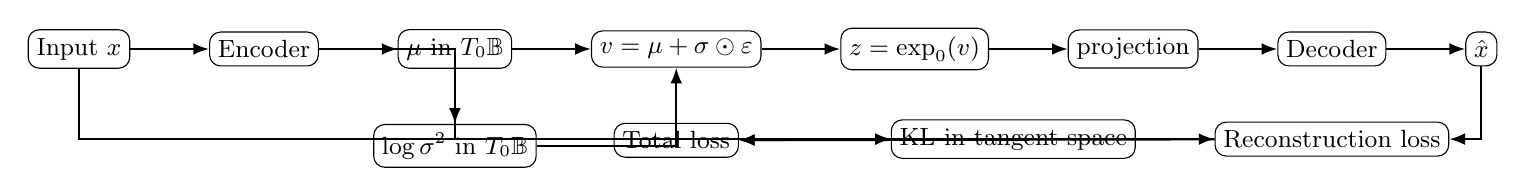
\begin{tikzpicture}[
  node distance=7mm and 10mm,
  box/.style={draw,rounded corners,align=center,inner sep=3pt,font=\small},
  arr/.style={-{Latex[length=2mm]},thick}
]
\node[box] (x) {Input $x$};
\node[box, right=of x] (enc) {Encoder};
\node[box, right=of enc] (mu) {$\mu$ in $T_0\mathbb B$};
\node[box, below=of mu] (lv) {$\log\sigma^2$ in $T_0\mathbb B$};
\node[box, right=of mu] (rep) {$v=\mu+\sigma\odot\varepsilon$};
\node[box, right=of rep] (exp) {$z=\exp_0(v)$};
\node[box, right=of exp] (proj) {projection};
\node[box, right=of proj] (dec) {Decoder};
\node[box, right=of dec] (xh) {$\hat x$};
\node[box, below=of dec] (rec) {Reconstruction loss};
\node[box, left=of rec] (kl) {KL in tangent space};
\node[box, below=of rep] (loss) {Total loss};

\draw[arr] (x) -- (enc);
\draw[arr] (enc) -- (mu);
\draw[arr] (enc) -| (lv);
\draw[arr] (mu) -- (rep);
\draw[arr] (lv) -| (rep);
\draw[arr] (rep) -- (exp);
\draw[arr] (exp) -- (proj);
\draw[arr] (proj) -- (dec);
\draw[arr] (dec) -- (xh);
\draw[arr] (xh) |- (rec);
\draw[arr] (x) |- (rec);
\draw[arr] (mu) |- (kl);
\draw[arr] (lv) |- (kl);
\draw[arr] (rec) -- (loss);
\draw[arr] (kl) -- (loss);
\end{tikzpicture}
\end{center}

\section{Remark}
The implementation adopts a practical tangent-space variational approximation rather than a fully manifold-native posterior/prior pair, trading exact geometric measure treatment for numerical stability and simpler optimization.

\end{document}
